% Uncomment this line for on-screen presentation
\documentclass[xcolor={dvipsnames}]{beamer}\usepackage{etoolbox}\newtoggle{printable}\togglefalse{printable}

% Uncomment this line for printable slides (disable animations and don't waste ink)
%\documentclass[handout, xcolor={dvipsnames}]{beamer}\usepackage{etoolbox}\newtoggle{printable}\toggletrue{printable}

% Adjust these for the path of the theme and its graphics, relative to this file
%\usepackage{beamerthemeFalmouthGamesAcademy}
\usepackage{../../beamerthemeFalmouthGamesAcademy}
\graphicspath{ {../../} }

% Default language for code listings
\lstset{language=C++,
		morekeywords={each,in}
}

\begin{document}
\title{Transition to C++ II}   
\subtitle{COMP110: Principles of Computing}

\frame{\titlepage} 

\begin{frame}{Learning outcomes}
	In this session you will learn how to...
	\begin{itemize}
		\item Split your program into multiple files, and understand the difference between
		    \textbf{source files} and \textbf{header files}
		\item Understand the C++ build pipeline, and the roles of the \textbf{preprocessor},
		    \textbf{compiler} and \textbf{linker}
		\item Use arrays, and the difference between creating them on the \textbf{stack}
		    versus on the \textbf{heap}
		\item Define C++ functions, and how passing \textbf{by reference} differs from passing \textbf{by value}
	\end{itemize}
\end{frame}

\part{Modular program design}
\frame{\partpage}

\begin{frame}[fragile]{Modular program design}
    \begin{itemize}
        \item We saw in session~9 that \textbf{splitting your code into several files} is generally a good idea \pause
        \item Python makes it easy: any .py file can be \lstinline[language=Python]{import}ed on demand \pause
        \item C++ is a little trickier...
    \end{itemize}
\end{frame}

\begin{frame}[fragile]{Definitions and declarations}
    A function \textbf{definition} specifies its name, return type, parameters, and the code it contains:
    \begin{lstlisting}
double average(double n1, double n2)
{
    return (n1 + n2) / 2.0;
}
    \end{lstlisting}
    \pause
    A function \textbf{declaration} specifies everything \textbf{except} the code:
    \begin{lstlisting}
double average(double n1, double n2);
    \end{lstlisting}
    \pause
    A declaration tells the compiler that this function exists, but is defined \textbf{elsewhere}
\end{frame}

\begin{frame}[fragile]{Sources and headers}
    \begin{itemize}
        \item A C++ project contains two main types of file \pause
        \item \textbf{Source files} (.cpp) usually contain \textbf{definitions} \pause
        \item \textbf{Header files} (.h) usually contain \textbf{declarations} \pause
        \item For example, \texttt{myfile.cpp} may contain some function definitions,
            and \texttt{myfile.h} may contain the declarations for those functions \pause
        \item (Yep, that means you have to type the same thing twice in two different files...)
    \end{itemize}
\end{frame}

\begin{frame}[fragile]{Example from last week}
    words.cpp
    \begin{lstlisting}
void readWords()
{
    std::cout << "Reading word list" << std::endl;
    // code omitted
}

std::string chooseRandomWord()
{
    // code omitted
}
    \end{lstlisting}
    
    words.h
    \begin{lstlisting}
#pragma once

void readWords();
std::string chooseRandomWord();
    \end{lstlisting}
\end{frame}

\begin{frame}[fragile]{Example from last week}
    \begin{itemize}
        \item \lstinline{readWords()} and \lstinline{chooseRandomWord()} are \textbf{defined} in \texttt{words.cpp} \pause
        \item \lstinline{readWords()} and \lstinline{chooseRandomWord()} are \textbf{declared} in \texttt{words.h} \pause
        \item Any file which does \lstinline{#include "words.h"} can call these functions as if they were declared in that file
    \end{itemize}
\end{frame}

\begin{frame}[fragile]{How \#include works}
    \begin{itemize}
        \item \lstinline{#include} works \textbf{exactly} as if the \lstinline{#include}d file were copied and pasted
            at the point where the \lstinline{#include} directive appears \pause
        \item All header files should start with \lstinline{#pragma once} --- otherwise,
            \lstinline{#include}ing the same file more than once will result in duplicate declaration errors \pause
        \item Putting an \lstinline{#include} directive in the wrong place (e.g.\ inside a function) will result in
            weird compile errors
    \end{itemize}
\end{frame}

\part{The build process}
\frame{\partpage}

\begin{frame}{Executing programs}
    \begin{itemize}
        \item CPUs execute \textbf{machine code} \pause
        \item Programs must be \textbf{translated} into machine code for execution \pause
        \item There are three main ways of doing this: \pause
        \begin{itemize}
            \item An \textbf{interpreter} is an application which reads the program source code and executes it directly \pause
            \item A \textbf{compiler} is an application which converts the program source code into executable machine code \pause
            \item A \textbf{just-in-time (JIT) compiler} is halfway between the two --- it compiles the program on-the-fly
                at runtime
        \end{itemize}
    \end{itemize}
\end{frame}

\begin{frame}{Examples}
	\begin{columns}[t,onlytextwidth]
		\begin{column}{0.3\textwidth}
		    Interpreted:
		    \begin{itemize}
		        \item Python
		        \item Lua
		        \item Bespoke scripting languages
		    \end{itemize}
		\end{column} \pause
		\begin{column}{0.3\textwidth}
		    Compiled:
		    \begin{itemize}
		        \item C
		        \item C++
		        \item Swift
		    \end{itemize}
		\end{column} \pause
		\begin{column}{0.3\textwidth}
		    JIT compiled:
		    \begin{itemize}
		        \item Java
		        \item C\#
		        \item JavaScript (in modern web browsers)
		        \item Jython
		    \end{itemize}
		\end{column}
	\end{columns}
\end{frame}

\begin{frame}{Interpreter vs compiler}
    \begin{itemize}
        \item Run-time efficiency: compiler $>$ interpreter \pause
        \begin{itemize}
            \item The compiler translates the program \textbf{in advance}, on the developer's machine \pause
            \item The interpreter translates the program \textbf{at runtime}, on the user's machine \pause
        \end{itemize}
        \item Portability: compiler $<$ interpreter \pause
        \begin{itemize}
            \item A compiled program can only run on the operating system and CPU architecture it was compiled for \pause
            \item An interpreted program can run on any machine, as long as a suitable interpreter is available \pause
        \end{itemize}
        \item JIT compilers have similar pros/cons to interpreters \pause
        \item For games, run-time efficiency is usually much more important than portability
    \end{itemize}
\end{frame}

\begin{frame}[fragile]{The C++ build process}
    \textbf{Preprocessor} \pause
    \begin{itemize}
        \item Replaces \lstinline{#include} directives with the contents of the appropriate header files \pause
        \item Handles other preprocessor directives (\lstinline{#define}, \lstinline{#if} etc --- more on these another time) \pause
    \end{itemize}
    \textbf{Compiler} \pause
    \begin{itemize}
        \item Translates each source file into an \textbf{object file} containing machine code \pause
    \end{itemize}
    \textbf{Linker} \pause
    \begin{itemize}
        \item Combines the object files together with any external libraries to produce an \textbf{executable}
            (on Windows, a .exe file)
    \end{itemize}
\end{frame}

\begin{frame}[fragile]{The C++ build process}
    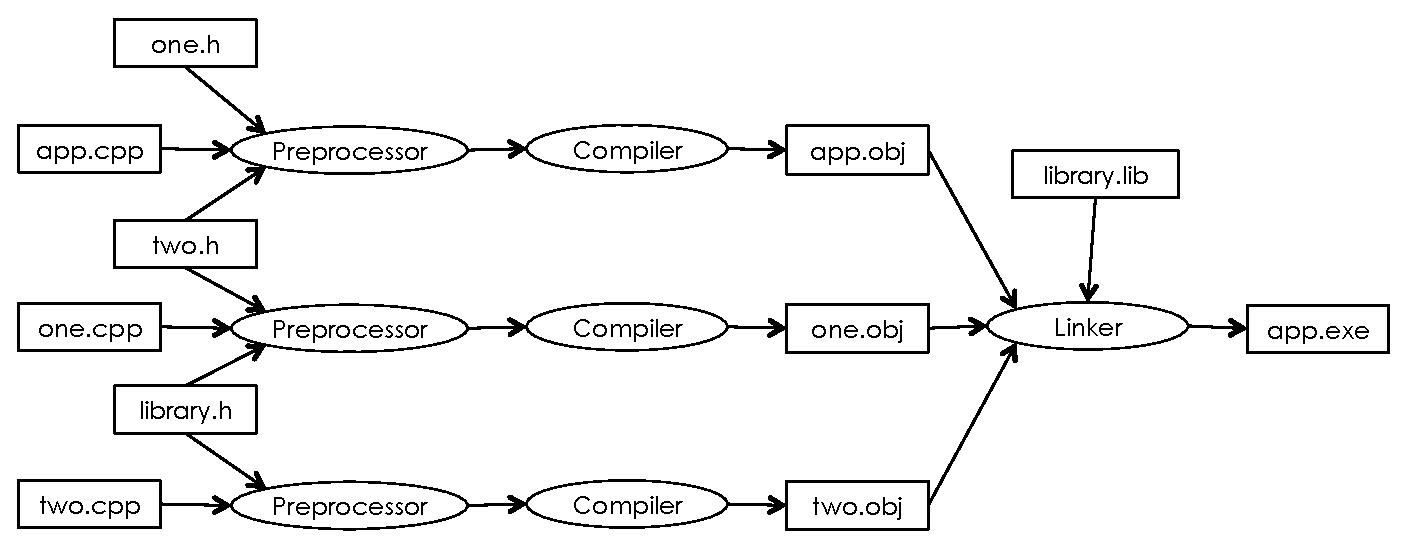
\includegraphics[width=\textwidth]{compiler_flowchart.pdf}
\end{frame}

\begin{frame}[fragile]{Modular design revisited}
    \begin{itemize}
        \item Your code can call any function for which there is a \textbf{declaration} in the current file
            (in the file itself or \lstinline{#include}d) \pause
        \item The \textbf{definition} of the function may be in another file \pause
        \item The \textbf{linker} resolves the function call in this case
    \end{itemize}
\end{frame}

\begin{frame}[fragile]{Incremental compilation}
    \begin{itemize}
        \item Compilation takes time --- compiling a AAA game can take several hours \pause
        \item Visual C++ stores intermediate files (e.g.\ \texttt{.obj} files) on disk \pause
        \item Only the changed files need to be run through the preprocessor and compiler again
            $\implies$ faster re-compilation during development \pause
        \item \textbf{Build $\to$ Clean} removes all intermediate files \pause
        \item \textbf{Build $\to$ Rebuild} forces Visual C++ to recompile everything
    \end{itemize}
\end{frame}

\begin{frame}[fragile]{Precompiled headers}
    \begin{itemize}
        \item Headers may need to be compiled multiple times if they are included in multiple source files \pause
        \item Headers may be very large ---
            e.g.\ \texttt{Windows.h} includes dozens of headers totalling many thousands of lines \pause
        \item In Visual C++ projects, \texttt{stdafx.h} is a \textbf{precompiled header} \pause
        \item \lstinline{#include "stdafx.h"} doesn't work like copy and paste ---
            instead, the compiler uses the precompiled header information \pause
        \item Precompiled header only needs to be recompiled if \texttt{stdafx.h} (or something it includes)
            changes, which should be rare
    \end{itemize}
\end{frame}

\begin{frame}[fragile]{Build configuration in VC++}
    \begin{center}
        
\includegraphics[width=0.6\textwidth]{vcpp_build_toolbar.PNG}
    \end{center}
     \pause
    \begin{itemize}
        \item Configuration:
        \begin{itemize}
            \item \textbf{Debug} allows use of the Visual C++ debugger \pause
            \item \textbf{Release} produces optimised code --- usually 2--10 $\times$ faster than Debug \pause
            \item Generally use Debug for development, Release for optimisation and distributing the finished application \pause
        \end{itemize}
        \item Platform:
        \begin{itemize}
            \item \textbf{x86} runs on 32-bit and 64-bit versions of Windows \pause
            \item \textbf{x64} runs on 64-bit Windows only \pause
            \item Generally use x86 for maximum compatibility, x64 for apps which need to use $>2$GB memory
                or where a significant speed benefit is measured
        \end{itemize}
    \end{itemize}
\end{frame}

\part{Basic containers in Python}
\frame{\partpage}

\begin{frame}{Memory allocation}
	\begin{itemize}
		\pause\item Memory is allocated in \textbf{blocks}
		\pause\item The program specifies the size, in bytes, of the block it wants
		\pause\item The OS allocates a \textbf{contiguous} block of that size
		\pause\item The program owns that block until it frees it
		\pause\item Forgetting to free a block is called a \textbf{memory leak}
			(not really possible in Python, but a common bug in C++)
		\pause\item Blocks can be allocated and deallocated at will, but can \textbf{never grow or shrink}
	\end{itemize}
\end{frame}

\begin{frame}{Containers}
	\begin{itemize}
		\pause\item Memory management is hard and programmers are lazy
		\pause\item Containers are an \textbf{abstraction}
			\begin{itemize}
				\pause\item Hide the details of memory allocation, and allow the programmer to write simpler code
			\end{itemize}
		\pause\item Containers are an \textbf{encapsulation}
			\begin{itemize}
				\pause\item Bundle together the data's representation in memory along with the algorithms for accessing it
			\end{itemize}
	\end{itemize}
\end{frame}

\begin{frame}{Arrays}
	\begin{itemize}
		\pause\item An \textbf{array} is a contiguous block of memory in which objects are stored,
			equally spaced, one after the other
		\pause\item Each array element has an \textbf{index}, starting from zero
		\pause\item Given the address of the $0$th element, it is easy to find the $i$th element:
	\end{itemize}
	$$ \text{address}_i = \text{address}_0 + (i \times \text{elementSize}) $$
	\begin{itemize}
		\pause\item E.g.\ if the array starts at address $1000$ and each element is $4$ bytes,
			the 3rd element is at address $1000 + 4 \times 3 = 1012$
		\pause\item Accessing an array element is \textbf{constant time} $O(1)$
	\end{itemize}
\end{frame}

\begin{frame}{Lists}
	\begin{itemize}
		\pause\item An array is a block of memory, so its size is \textbf{fixed} once created
		\pause\item A \textbf{list} is a variable size array
		\pause\item When the list needs to change size, it \textbf{creates} a new array,
			\textbf{copies} the contents of the old array, and \textbf{deletes} the old array
		\pause\item Implementation details: \url{http://www.laurentluce.com/posts/python-list-implementation/}
	\end{itemize}
\end{frame}

\begin{frame}{Time taken to append an element to a list of size $n$}
	\begin{center}
		\vspace{-5ex}
		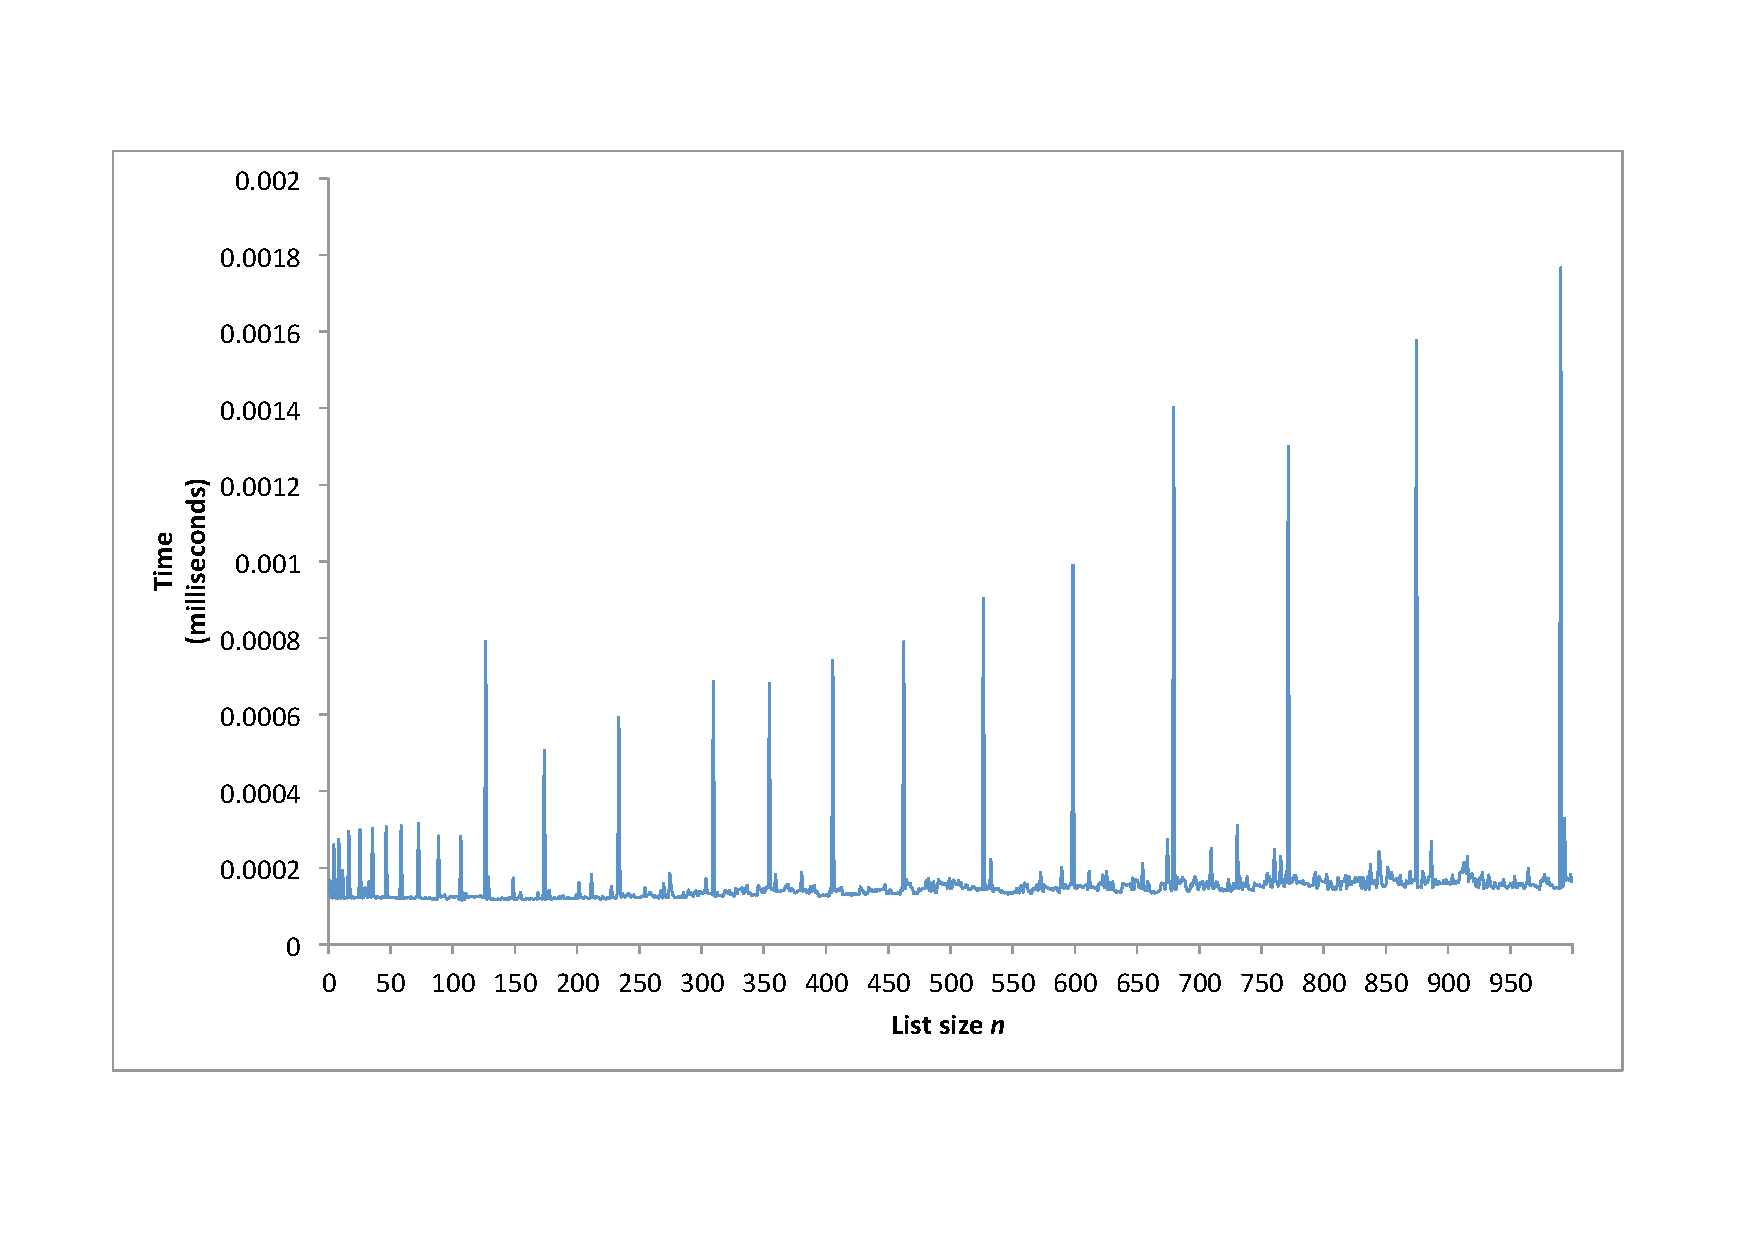
\includegraphics[height=0.9\textheight]{list_append_timing}
	\end{center}
\end{frame}

\begin{frame}{Operations on lists}
	\begin{itemize}
		\pause\item \textbf{Appending} to a list is \textbf{amortised constant time}
			\begin{itemize}
				\pause\item Usually $O(1)$, but can go up to $O(n)$ if the list needs to change size
			\end{itemize}
		\pause\item \textbf{Inserting} anywhere other than the end is \textbf{linear time}
			\begin{itemize}
				\pause\item Can't just insert new bytes into a memory block ---
					need to move all subsequent list elements to make room
			\end{itemize}
		\pause\item Similarly, \textbf{deleting} anything other than the last element is \textbf{linear time}
	\end{itemize}
\end{frame}

\begin{frame}{Tuples}
	\begin{itemize}
		\pause\item Tuples are like lists, but are \textbf{immutable}
			\begin{itemize}
				\pause\item Read-only
				\pause\item Once created, can't be changed
			\end{itemize}
		\pause\item Useful for storing sequences of values where adding, inserting, deleting or
			changing individual values does not make sense
			\begin{itemize}
				\pause\item E.g.\ $xy$ coordinates, RGB colours, ...
			\end{itemize}
		\pause\item Create tuples with \lstinline{()}, just as you create lists with \lstinline{[]}
			\begin{itemize}
				\pause\item Exception: a single element tuple is created as \lstinline{(foo,)}
					because \lstinline{(foo)} would be interpreted as a bracketed expression
			\end{itemize}
		\pause\item Can often omit the parentheses entirely, e.g.\ \lstinline{my_tuple = 1,2,3}
	\end{itemize}
\end{frame}

\begin{frame}[fragile]{Unpacking}
	If \lstinline{foo} is a list or tuple of length 4, the following are equivalent:
	\pause
	\begin{columns}
		\begin{column}{0.48\textwidth}
			\begin{lstlisting}
a, b, c, d = foo
			\end{lstlisting}
		\end{column}
		\pause
		\begin{column}{0.48\textwidth}
			\begin{lstlisting}
a = foo[0]
b = foo[1]
c = foo[2]
d = foo[3]
			\end{lstlisting}
		\end{column}
	\end{columns}
	\begin{itemize}
		\pause\item Unpacking requires the number of elements to match exactly ---
			if \lstinline{foo} has more than 4 elements, the code on the left will give an error
	\end{itemize}
\end{frame}

\begin{frame}[fragile]{One weird trick (Java programmers hate it!)}
	The following are equivalent:
	\pause
	\begin{columns}
		\begin{column}{0.48\textwidth}
			\begin{lstlisting}
a, b = b, a
			\end{lstlisting}
		\end{column}
		\pause
		\begin{column}{0.48\textwidth}
			\begin{lstlisting}
temp = a
a = b
b = temp
			\end{lstlisting}
		\end{column}
	\end{columns}
\end{frame}

\begin{frame}[fragile]{Strings are immutable}
	\begin{itemize}
		\pause\item \textbf{Strings} are immutable in Python
			\begin{itemize}
				\pause\item This is not true of all programming languages
			\end{itemize}
		\pause\item But wait... we change strings all the time, don't we?
	\end{itemize}
	\begin{lstlisting}
my_string = "Hello "
my_string += "world"
	\end{lstlisting}
	\begin{itemize}
		\pause\item This isn't changing the string, it's creating a new one and throwing the old one away!
		\pause\item Hence building a long string by appending can be slow (appending strings is $O(n)$)
	\end{itemize}
\end{frame}

\begin{frame}{Dictionaries}
	\begin{itemize}
		\pause\item Dictionaries are \textbf{associative maps}
		\pause\item A dictionary maps \textbf{keys} to \textbf{values}
			\begin{itemize}
				\pause\item Keys must be immutable (numbers, strings, tuples etc)
				\pause\item Values can be anything (including dictionaries or other containers)
			\end{itemize}
		\pause\item A dictionary is implemented as a \textbf{hash table}
	\end{itemize}		
\end{frame}

\begin{frame}[fragile]{Using dictionaries}
	\pause Create them using \lstinline|{}|:
	\begin{lstlisting}
age = {"Alice": 23, "Bob": 36, "Charlie": 27}
	\end{lstlisting}
	\pause Access values using \lstinline{[]}:
	\begin{lstlisting}
print(age["Alice"]) # prints 23
age["Bob"] = 40     # overwriting an existing item
age["Denise"] = 21  # adding a new item
	\end{lstlisting}
\end{frame}

\begin{frame}[fragile]{Iterating over dictionaries}
	\pause Iterating over a dictionary gives the \textbf{keys}:
	\begin{lstlisting}
for x in age:
    print(x)   # prints Alice, Bob, Charlie
	\end{lstlisting}
	\pause Use \lstinline{items} to get \textbf{key,value} pairs:
	\begin{lstlisting}
for key, value in age.items():
    print(key, "is", age, "years old")
	\end{lstlisting}
\end{frame}

\begin{frame}{Sets}
	\begin{itemize}
		\pause\item Sets are like dictionaries without the values
		\pause\item Sets are \textbf{unordered} collections of \textbf{unique} elements
            \begin{itemize}
                \pause\item Sets \textbf{cannot} contain \textbf{duplicate} elements
                \pause\item Attempting to \lstinline{add} an element already present in the set does nothing
            \end{itemize}
		\pause\item Certain operations on sets scale better on average than the equivalent operations on lists:
	\end{itemize}
	\pause
	\begin{center}
		\begin{tabular}{|c|c|c|}
			\hline
			\textbf{Operation} & \textbf{List} & \textbf{Set} \\\hline
			Add element & Append: $O(1)$ & $O(1)$ \\
			& Insert: $O(n)$ & \\\hline
			Delete element & $O(n)$ & $O(1)$ \\\hline
			Contains element? & $O(n)$ & $O(1)$ \\\hline
		\end{tabular}
	\end{center}
\end{frame}

\begin{frame}[fragile]{Using sets}
    \pause Create them using \lstinline|{}|:
	\begin{lstlisting}
numbers = {1, 4, 9, 16, 25}
	\end{lstlisting}
	\pause Add and remove members with \lstinline{add} and \lstinline{remove} methods
	\begin{lstlisting}
numbers.add(36)
numbers.remove(4)
	\end{lstlisting}
	\pause Test membership with \lstinline{in} operator
	\begin{lstlisting}
if 9 in numbers:
    print("Set contains 9")
	\end{lstlisting}
\end{frame}

\part{Functions}
\frame{\partpage}

\begin{frame}[fragile]{Function definitions}
    \begin{itemize}
        \item We have already seen an example of a function definition
    \end{itemize}
    \begin{lstlisting}
int main()
{
    std::cout << "Hello, world!" << std::endl;
    return 0;
}
    \end{lstlisting}
    \begin{itemize}
        \item The function \lstinline{main} takes no parameters, and returns a value of type \lstinline{int}
    \end{itemize}
\end{frame}

\begin{frame}[fragile]{Function signatures}
    \begin{itemize}
        \item The \textbf{signature} of a function defines its return type, name, and parameters
    \end{itemize}
    \begin{lstlisting}
double foo(std::string x, int y, bool z)
    \end{lstlisting}
    \pause
    \begin{itemize}
        \item This function takes three parameters: \pause
        \lstinline{x} of type \lstinline{std::string}, \pause
        \lstinline{y} of type \lstinline{int}, \pause
        and \lstinline{z} of type \lstinline{bool} \pause
        \item It returns a value of type \lstinline{double}
    \end{itemize}
\end{frame}

\begin{frame}[fragile]{Functions without return values}
    \begin{itemize}
        \item It is possible to define a function which does not return a value, using the \lstinline{void} keyword
        in place of its return type
    \end{itemize}
    \pause
    \begin{lstlisting}
void printNumber(int n)
{
    std::cout << n << std::endl;
}
    \end{lstlisting}
\end{frame}

\begin{frame}[fragile]{Pass by value}
    \begin{itemize}
        \item Function parameters are passed \textbf{by value}:
        the function receives \textbf{copies} of the original variables
    \end{itemize}
    \pause
    \begin{lstlisting}
void changeName(std::string name)
{
    name = "Ed";
}

int main()
{
    std::string name = "Mike";
    std::cout << name << std::endl; // Mike
    changeName();
    std::cout << name << std::endl; // Mike
}
    \end{lstlisting}
\end{frame}

\begin{frame}[fragile]{Pass by reference}
    \begin{itemize}
        \item Parameters can be passed \textbf{by reference} using \lstinline{&}, allowing the function to modify them
    \end{itemize}
    \pause
    \begin{lstlisting}
void changeName(std::string& name)
{
    name = "Ed";
}

int main()
{
    std::string name = "Mike";
    std::cout << name << std::endl; // Mike
    changeName();
    std::cout << name << std::endl; // Ed
}
    \end{lstlisting}
\end{frame}

\begin{frame}[fragile]{One area where C++ is ``simpler'' than Python!}
    \begin{itemize}
        \item Recall from COMP110 week 6: in Python, basic data types (numbers, booleans, strings etc)
            are passed by value, and object types (lists, dictionaries, class instances) are passed by reference
        \pause
        \item In C++, everything is passed by value unless it is explicitly marked as a reference with \lstinline{&}
    \end{itemize}
\end{frame}

\begin{frame}[fragile]{Constant references}
    \begin{lstlisting}
void greet(std::string name)
{
    std::cout << "Hi " << name << std::endl;
}
    \end{lstlisting}
    \pause
    \begin{itemize}
        \item The string will be copied in order to be passed in \pause
        \item More efficient to pass a reference, and mark it \lstinline{const} to prevent accidental modification
    \end{itemize}
    \begin{lstlisting}
void greet(const std::string& name)
{
    std::cout << "Hi " << name << std::endl;
}
    \end{lstlisting}
    \pause
    \begin{itemize}
        \item (this is only worthwhile for large data structures like strings and vectors, not for basic data types)
    \end{itemize}
\end{frame}



\part{Live coding: Noughts and Crosses}
\frame{\partpage}

% -------------------------------------------------------

%\part{The compiler}
%\frame{\partpage}
%
%\begin{frame}
%	\frametitle{The build process}
%	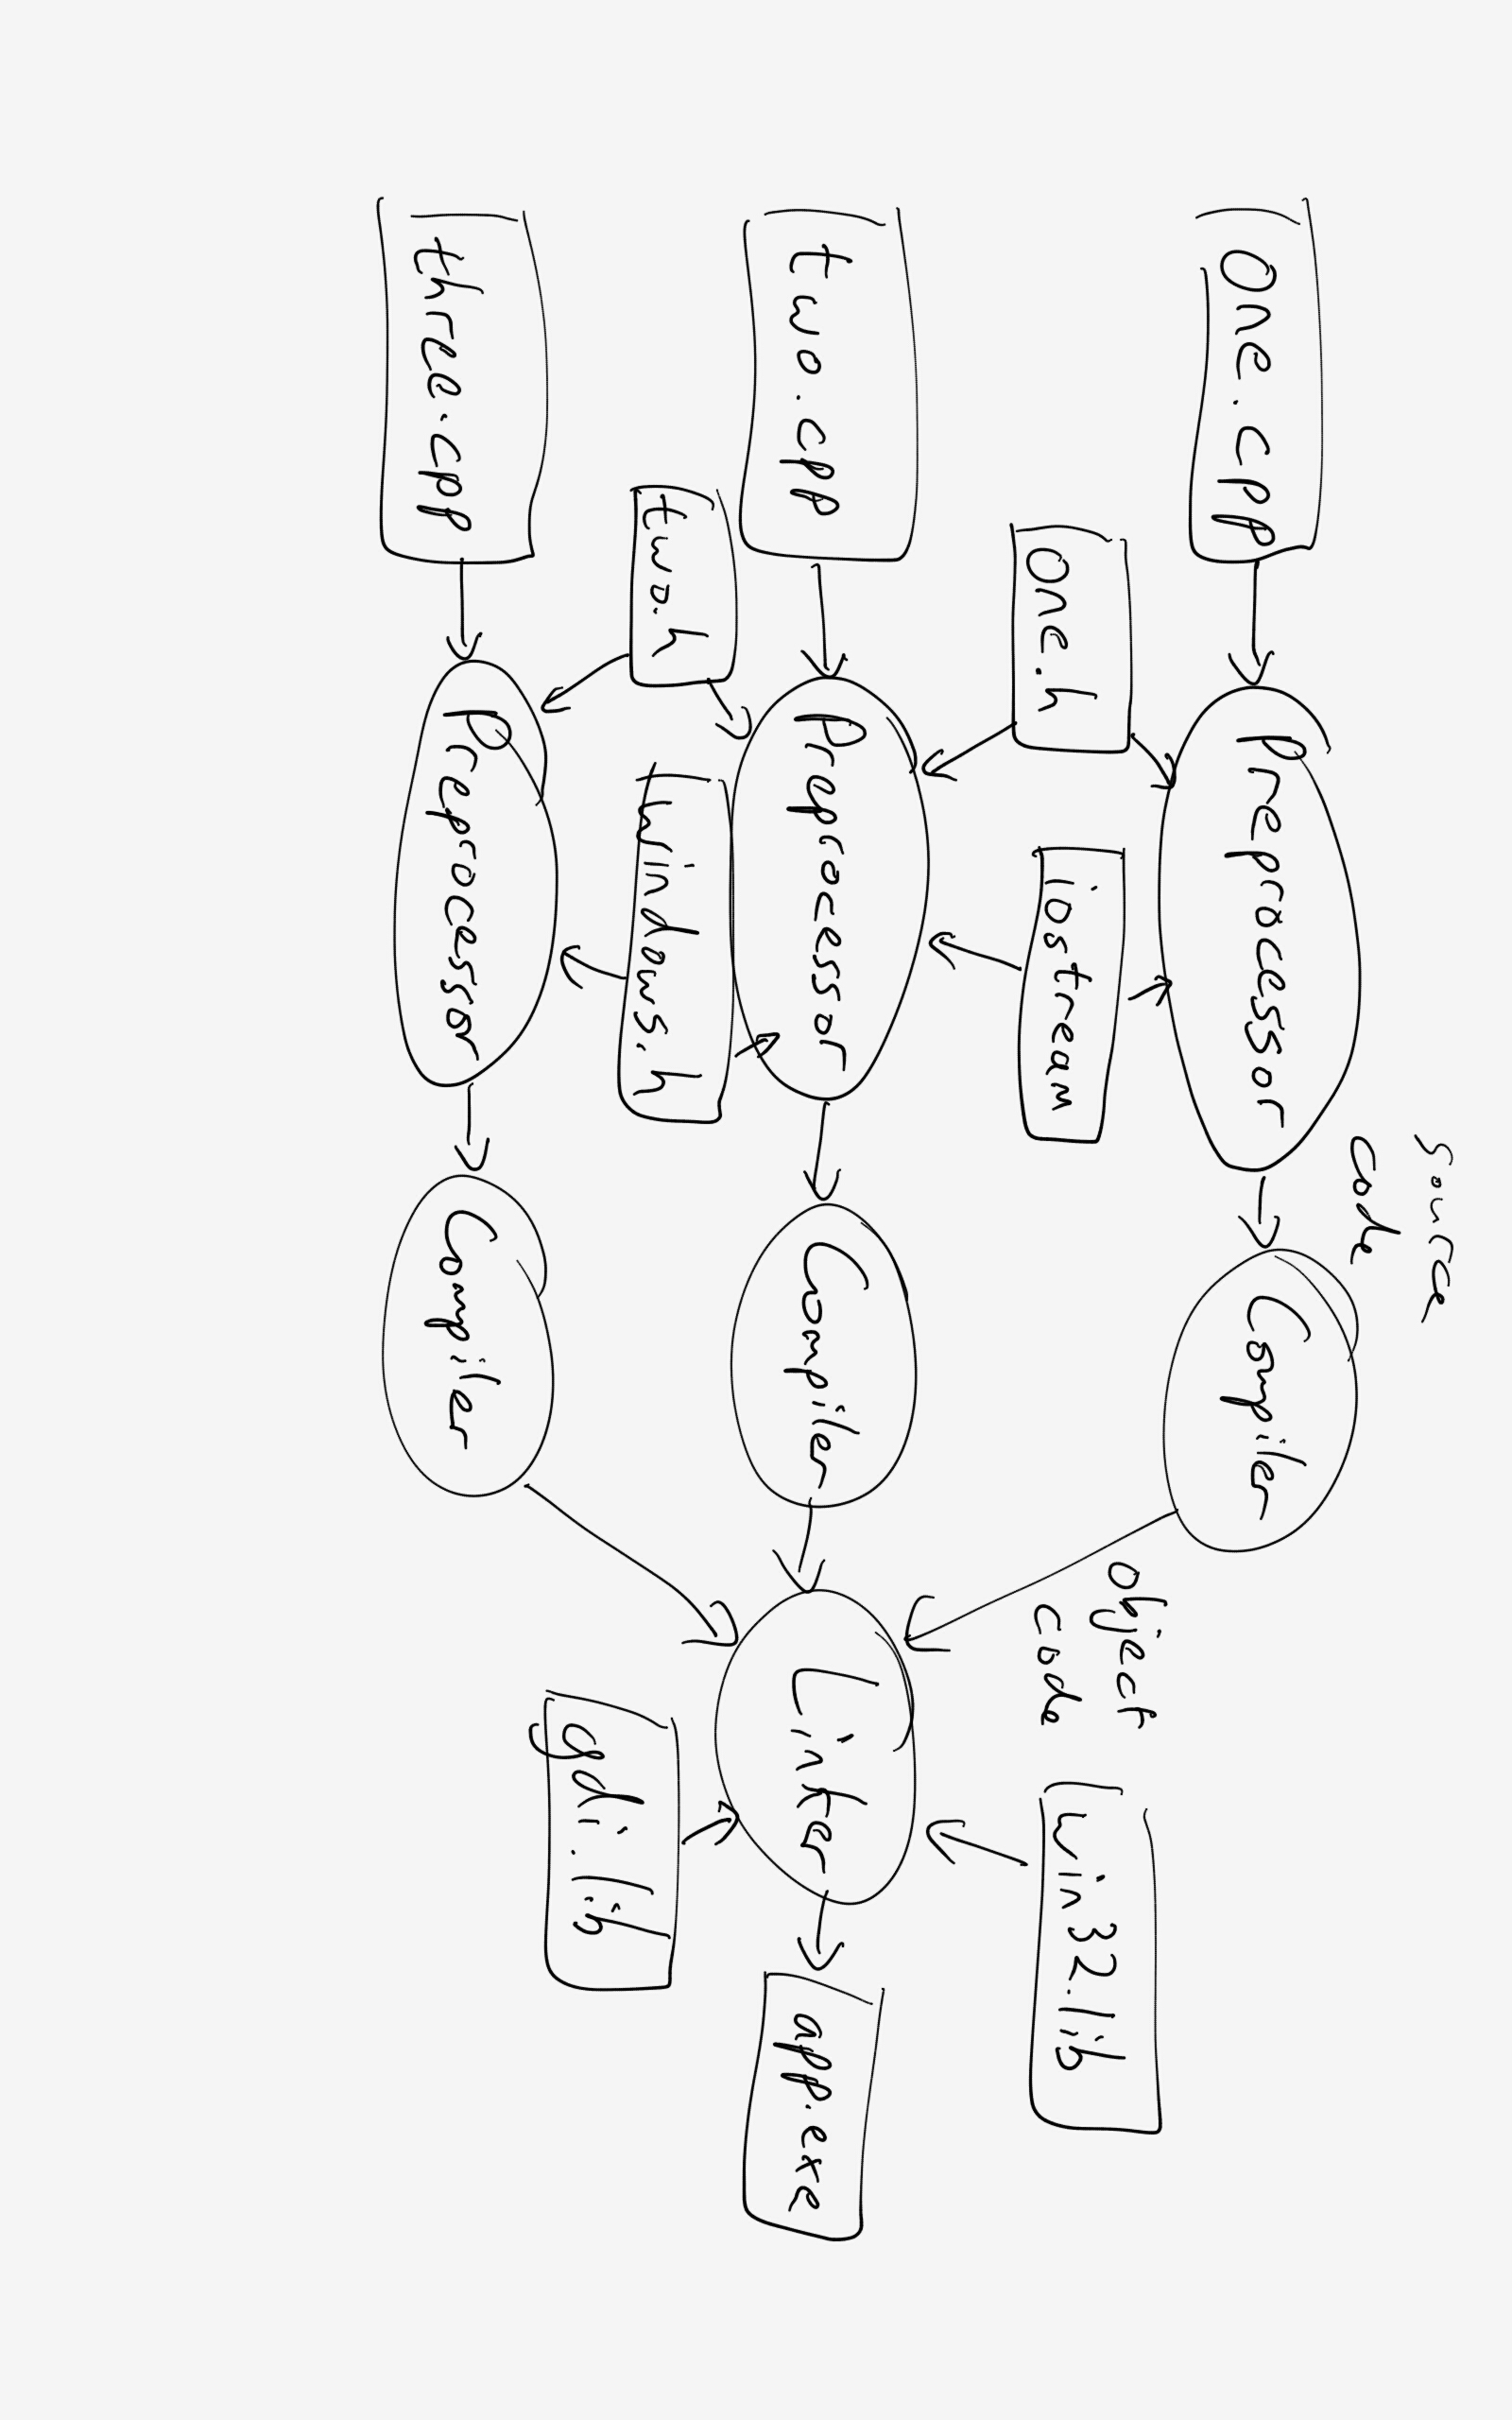
\includegraphics[height=\textwidth,angle=90]{compiler_sketch}
%\end{frame}

\end{document}
